\subchapter{Bootloader - U-Boot}{Objectives: Compile and install the U-Boot bootloader, 
  use basic U-Boot commands, set up TFTP communication with the development
  workstation.}

As the bootloader is the first piece of software executed by a
hardware platform, the installation procedure of the bootloader is
very specific to the hardware platform. There are usually two cases:

\begin{itemize}

\item The processor offers nothing to ease the installation of the
  bootloader, in which case the JTAG has to be used to initialize
  flash storage and write the bootloader code to flash. Detailed
  knowledge of the hardware is of course required to perform these
  operations.

\item The processor offers a monitor, implemented in ROM, and through
  which access to the memories is made easier.

\end{itemize}

The \devboard board, which uses an AM335x Sitara processor, falls into
the second category. 

The Sitara processors support a multitude of boot sources, and the boot
source is selected by configuring a set of pins at reset.
The Beaglebone limits the choices to one of two options and you choose
which one, with a button.

The monitor integrated in the ROM reads the internal
eMMC flash chip to search for a valid bootloader.
If the user button is pressed at reset, the Sitara processor will instead search
for a micro-SD card inserted in the connector.

The U-Boot bootloader programmed into the Beaglebone Black boots linux
by executing the contents of the "bootcmd" environment variable, 
which normally tries to use the SD-Card contents first, and the eMMC memory
only if booting from SD-Card fails, so normally the button does not have to be pressed.


\clearpage
\section{Setup}

Go to the \labdir directory and the enter the \code{bootloader} subdirectory.

\section{U-Boot setup}

Download U-Boot from the mainline U-Boot download site:

\begin{verbatim}
wget ftp://ftp.denx.de/pub/u-boot/u-boot-2013.10.tar.bz2
tar -jxvf u-boot-2013.10.tar.bz2
cd u-boot-2013.10
\end{verbatim}

We want to figure out what is going on, so we will init a git repo.

Then we will add all the files and create a commit.

\begin{verbatim}
git init
git add .
git commit -m "Initial Commit" -s
\end{verbatim}

The '-m' switch will tell git to use the following string as the commit message,
and the '-s' switch will sign the commit with your user info as defined above.

We will apply two patches that are in the \code{data} directory that needs to be applied.

\begin{itemize}
\item \code{0001-arm-omap-i2c-don-t-zero-cnt-in-i2c_write.patch}
	This is a minor fix for a device driver.

\item \code{0002-Read-environment-from-uSetup.txt-at-boot-if-present.patch}
	This is a fix which adds a significant functionality to the bootloader
	and is neccessary for the labs.

\end{itemize}

The traditional way is to \code{'cat'} the patch and pipe it through the \code{'patch'} utility,
but we will do it using git instead

Example: Applying a patch in the traditional Way:
{\small
\begin{verbatim}
cat /path/to/0001-arm-omap-i2c-don-t-zero-cnt-in-i2c_write.patch | \
   patch -p1
\end{verbatim}
}

Example: applying a patch using git:

{\small
\begin{verbatim}
git am /path/to/0001-arm-omap-i2c-don-t-zero-cnt-in-i2c_write.patch
\end{verbatim}
}

\code{'git am'} will not only apply the patch, it will also commit the patch
using the original patch message. There are more requirements on a patch
when you use "git am", since it will only accept well formed patches.

If a patch fails, then it will give you different options on how to handle the problem.

Apply the patch.

\begin{verbatim}
cd u-boot-2013.10
git am ../data/*.patch
\end{verbatim}

Patching with ''git am' should succeed, if you did not patch using the traditional way first.

If it fails, you can abort the patch through:
{\small
\begin{verbatim}
git am --abort
\end{verbatim}
}

You can check the status of the git tree. Try:
{\small
\begin{verbatim}
git status
\end{verbatim}
}

If you see any modified files, you can restore them using the checkout command.

{\small
\begin{verbatim}
git checkout <filename>
\end{verbatim}
}

This will restore the file to its original state.

Try out:
{\small
\begin{verbatim}
git log
\end{verbatim}
}

\clearpage
\section{U-Boot Source Tree}
Get an understanding of U-Boot's configuration and compilation steps by
reading the \code{README} file, and specifically the {\em Building the
  software} section.

Basically, you need to:

\begin{itemize}
\item set up the cross compiler (You could source the \code{toolchain.sh} script in the top directory)
or if you use the Yocto toolchain, source the appropriate \code{environment...} file
\begin{verbatim}
#!/bin/sh
export	ARCH=arm
export	GCCROOT=/usr/local/uclibc/arm-unknown-linux-uclibcgnueabihf
export	PATH=$GCCROOT/bin:$PATH
export	CROSS_COMPILE=arm-linux-
\end{verbatim}

\item Configure U-Boot to build for the Beaglebone Black

Note that for our platform, the configuration file is
\begin{verbatim}
include/configs/am335x_evm.h
\end{verbatim}
Read this file to get an
  idea of how a U-Boot configuration file is written;

Then configure U-Boot.

\begin{verbatim}
$ make am335x_boneblack_config
Configuring for am335x_boneblack - Board: am335x_evm, Options: SERIAL1,CONS_INDEX=1,EMMC_BOOT
\end{verbatim}

If you get a lot of errors, try \code{make clean} or \code{make distclean} and rerun.


You should see something similar to:
\begin{verbatim}
Configuring for am335x_boneblack - Board: am335x_evm,
    Options: SERIAL1,CONS_INDEX=1,EMMC_BOOT
\end{verbatim}

This configuration step generates a \code{Makefile} fragment which you may want to look at.

\begin{verbatim}
include/autoconf.mk
\end{verbatim}

\item Finally, run \code{make}\footnote{You can speed up the compiling
  by using the \code{-jX} option with \code{make}, where X is the number of parallel
  jobs used for compiling. Twice the number of CPU cores is a good
  value.}, which should build U-Boot.

\end{itemize}

One would think that the build generated a number of new files. Checking with:

{\small
\begin{verbatim}
git status
\end{verbatim}
}

should print out:

\begin{verbatim}
# On branch master
nothing to commit (working directory clean)
\end{verbatim}

If you do an \code{ls} you {\bf will} see some new files like \code{u-boot.img}.

The reason they are not detected, is that they are hidden by the \code{.gitignore} file 
filter. If you name a \code{regexp} in \code{.gitignore} it will be ignored.

List the \code{.gitignore} by \code{more .gitignore}.

\section{Rescue binaries}

If you have trouble generating binaries that work properly, or later
make a mistake that causes you to loose your \code{MLO} and
\code{u-boot.img} files, you will find working versions under
\code{data/} in the current lab directory.

\clearpage

\section{The U-Boot boot process}

When U-Boot starts, it loads the environment from a non-volatile memory to RAM
The environment is a set of variables, which can be used as scripts through the \code{run}
command. Other environment variables are used to define constants like addresses,
for use in script variables

The location of the environment memory is defined in a compile time constant,
typically set in \code{board.cfg}.
Examples of environment memory types are NOR Flash, NAND Flash, SPI Flash and I2C EEPROM.

The first time U-Boot is started on a board, it will load a default environment.

You can modify a variable or create a new one with the \code{setenv} command.

If you have an environment memory, you can save the updated environment with the \code{saveenv} command.

The next time, U-boot is started, it will detect that you have a valid environment,
and load this, instead of the default environment.

Not every board has an environment memory, and an example of the this is the \devboard.
Such board will always load the default memory at start-up. 

The U-Boot process depends on two special variables \code{bootcmd} and \code{bootargs}.

If the user does not intervene, by pressing \code{<return>}, U-Boot will \code{run}
the \code{bootcmd} variable script.  Typically the last command executed in \code{bootcmd}
is a command which boots the linux kernel.  There are several commands available.

\begin{itemize} 

\item \code{bootm} Boots a \code{uImage}

\item \code{bootz} Boots a \code{zImage}

\end{itemize}

When any of the boot commands are executed, they will boot the kernel and pass
the contents of the \code{bootargs} variable to the kernel.

The way to use the U-Boot environment has been refined over time. In early days,
you would typically set the \code{bootargs} directly. The current approach is
to run a variable script which generates \code{bootargs} from a set of other variables.

More information about U-Boot is available in \code{http://www.denx.de/wiki/DULG/Manual}

The \devboard predefined environment is set-up to boot from an SD-Card.

The \devboard \code{bootcmd} is fairly complex, and tries to detect an external SD-Card.
If not present, it will use the soldered SD-Card.
Once the card is selected, U-Boot will try to load the file \code{uEnv.txt}
and import the contents into the environment.

The syntax for setting variables in \code{uEnv.txt} are

\begin{verbatim}
<VARIABLE>=<VALUE>
\end{verbatim}

An Example:

\begin{verbatim}
uenvcmd=run tftp_kernel tftp_dtb netargs bootkernel
\end{verbatim}

This creates the variable script \code{uenvcmd} to run four scripts in succession.

The variable \code{uenvcmd} has a special meaning in the \devboard U-Boot.
Once the \code{uEnv.txt} has been imported, \code{bootcmd} will test
for the precense of this variable, and if it exists, it will be \code{run}.

By setting this to a suitable value, you can boot from any source.

If \code{uenvcmd} is not defined in \code{uEnv.txt}, 
U-Boot will try to load the kernel and device-tree file
from the second partition of the SD-Card which
normally should contain the file system.
The default assumes that they are located in the \code{/boot} directory.

It will set-up the \code{bootargs} variable to use the second partition
of the SD-Card as its root and then boot the kernel.

There is a small problem with this approach, and that it does 
not give the user any flexibility. If the boot is stopped before
\code{bootcmd} is executed, only the default environment is available.

If \code{bootcmd} is executed, it cannot easily be stopped, so while
U-Boot can be booted from any source, it boot sequence cannot be changed
without modifying the \code{uEnv.txt} file.

The patched U-Boot used in this lab, supports an alternative method.

\section{The U-Boot modified boot process}

After U-Boot has loaded the default environment, it will load the \code{uSetup.txt}
file from the seclected SD-Card and import its content into the environment. It has the same syntax as the \code{uEnv.txt} file.
This happens before U-Boot checks if the user wants to abort the automatic boot,
by pressing \code{<return>} key.

If the user does not abort, the \code{bootcmd} command will be executed.

By changing the \code{bootcmd} command in \code{uSetup.txt}, you can make U-Boot
boot from any source.

If the user aborts the automatic boot, and enters the U-Boot command loop,
\code{uSetup.txt} can have created scripts, that can be run manually,
to allow easy selection of the boot sequence.

\section{Preparing an SD-card with U-Boot}

Copy the generated \code{MLO} and \code{u-boot.img} files
to the SD card FAT partition. \code{MLO} is the first stage bootloader,
\code{u-boot.img} is the second stage bootloader.

\clearpage

\section{Preparing an SD-card with U-Boot using uEnv.txt}

We will create a new \code{uEnv.txt} on the host using the template below.

Change values to fit your setup:

You should use the same values for {\bf ipaddr} and {\bf serverip} as used in the toplevel \code{host.mk} file.

\fbox{\begin{minipage}{\textwidth}
{\bfseries
Caution:  For technical reasons, long lines are split up in this pdf file, 
using the {\bf \code{'\'}} character. In the \code{uEnv.txt} file, they must be a single line with the {\bf \code{'\'}} character removed.
}
\end{minipage}}

\begin{verbatim}
tftp_dtb=tftp ${fdtaddr} \
  am335x-boneblack.dtb
\end{verbatim}

should look like

\begin{verbatim}
tftp_dtb=tftp ${fdtaddr} am335x-boneblack.dtb
\end{verbatim}

in the file.

\fbox{\begin{minipage}{\textwidth}
{\bfseries
Variables using split lines like this are 'netargs'
}
\end{minipage}}


\begin{verbatim}
ipaddr=192.168.0.100
serverip=192.168.0.1
loadaddr=0x80200000
fdtaddr=0x80F80000
IMAGE=rootfs
console=ttyO0,115200n8
nfsopts=nolock
netargs=setenv bootargs console=${console} root=/dev/nfs \
  nfsroot=${serverip}:/tftpboot/${IMAGE},${nfsopts} rw ip=${ipaddr}
tftp_kernel=tftp ${loadaddr} zImage
tftp_dtb=tftp ${fdtaddr} am335x-boneblack.dtb
bootkernel=bootz ${loadaddr} - ${fdtaddr}
uenvcmd=run tftp_kernel tftp_dtb netargs bootkernel
mmcboot=echo MMC boot disabled
nandboot=echo NAND boot disabled
\end{verbatim}

\fbox{\begin{minipage}{\textwidth}
{\bfseries
Caution: In \code{ttyO2}, it's the capital letter \code{O}, like in {\bf O}MAP and not the number zero)
}
\end{minipage}}

Copy the file to the FAT partition.

Create an empty file \code{uSetup.txt} in the same place. 

Remember to run \code{sudo sync} before unmounting and removing the card.

\clearpage
\section{Preparing an SD-card with U-Boot using uSetup.txt}

Our U-Boot patch (which is not standard) will start by reading the \code{uSetup.txt}
before \code{bootcmd} is executed, so you have a chance to stop the boot,
by pressing {\bf return}.

Below is a template for the file \code{uSetup.txt}, but it needs to be edited
before it can be used. 

Create a \code{uSetup.txt} file on your host.

You should use the same values for {\bf ipaddr} and {\bf serverip} as used in the toplevel \code{host.mk} file.

\fbox{\begin{minipage}{\textwidth}
{\bfseries
Caution:  For technical reasons, long lines are split up in this pdf file, 
using the {\bf \code{'\'}} character. In the \code{uEnv.txt} file, they must be a single line with the {\bf \code{'\'}} character removed.
}
\end{minipage}}

{\bf The assignments of 'netargs' and 'mmcargs' should each be a single line.}

In \code{ttyO2}, it's the capital letter \code{O}, like in {\bf O}MAP and not the number zero)

\begin{verbatim}
ipaddr=192.168.0.100
serverip=192.168.0.1
loadaddr=0x80200000
fdtaddr=0x80F80000
IMAGE=rootfs
console=ttyO0,115200n8
nfsopts=nolock
netargs=setenv bootargs console=${console} root=/dev/nfs \
  nfsroot=${serverip}:/tftpboot/${IMAGE},${nfsopts} rw ip=${ipaddr}
tftp_kernel=tftp ${loadaddr} zImage
tftp_dtb=tftp ${fdtaddr} am335x-boneblack.dtb
bootkernel=bootz ${loadaddr} - ${fdtaddr}
mmcargs=setenv bootargs console=${console} ${optargs} root=${mmcroot} \
  rootfstype=${mmcrootfstype} rootwait
mmcrootfstype=squashfs
nandboot=echo NAND boot disabled
bootcmd=run tftp_kernel tftp_dtb netargs bootkernel
\end{verbatim}

Do not copy \code{uSetup.txt} to the SD-Card yet, instead keep the empty 
\code{uSetup.txt} in the FAT partition.

\clearpage

\section{Testing U-Boot on the MMC card}

Insert the MMC card into the Beaglebone Black board, Unplug the power cord.
While pressing the user button, reinsert the power cord and check that it boots your new bootloader. 
You can verify this by checking the build date: (Should obviously be todays date). 
Press the {\bf RETURN} button, when the prompt says \code{Hit anykey to stop autoboot:}

\begin{center}
    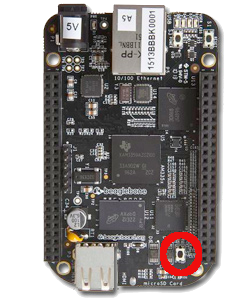
\includegraphics[height=5cm]{labs/sysdev-u-boot-BBB/beagleboneblack-user-button.png}
\end{center}

If the SD-Card boot does not work, the processor will try to boot from the internal eMMC memory,
and the date will be different from todays date.

If that happens, retry removing the power plug, then push the button, reinsert power.

If it still does not work , verify that the SD card is correctly setup using \code{cfdisk} 

\begin{itemize}
\item heads=255
\item sectors=63
\item partition 1 is bootable
\item partition 1 is FAT formated and contains \code{MLO}, \code{u-boot.img} and \code{uEnv.txt}
\end{itemize}


\clearpage

If it works you will see something similar to:

\begin{verbatim}
U-Boot SPL 2013.10-gbd39439-dirty (Mar 03 2014 - 18:03:52)
spl: error reading image args, err - 0
reading u-boot.img


U-Boot 2013.10-gbd39439-dirty (Mar 03 2014 - 20:04:45)

I2C:   ready
DRAM:  512 MiB
WARNING: Caches not enabled
MMC:   OMAP SD/MMC: 0, OMAP SD/MMC: 1
Using default environment

Net:   <ethaddr> not set. Validating first E-fuse MAC
cpsw, usb_ether
Hit any key to stop autoboot:  0 
\end{verbatim}

The message \code{reading u-boot.img} also confirms that U-Boot has
been loaded from the MMC device. The error message is due to the \code{Falcon mode} which
will allow booting the kernel directly from \code{MLO} without loading U-Boot. We do not use this mode.

When U-Boot initializes, it will execute the contents of the \code{bootcmd} variable as a script.

Before that happens, it will wait for a few seconds (value of \code{bootdelay}) giving
the user a chance to stop the boot. 

Press the \code{<return>} button before the counter expires, to enter the U-Boot shell.

(You may have to reset the Beaglebone if you did not manage to press the \code{<return>} button in time)
\begin{verbatim}
U-Boot #
\end{verbatim}

In U-Boot, type the \code{help} command, and explore the few commands available.

You can get more help on a specific command. Try \code{help boot}.

\clearpage

\section{The Default U-Boot Environment}
U-Boot supports an environment, and you can extend the commandset by defining environment variables.
These can be "used" as scripts through the \code{run} command 
It is possible to define a compile time environment, which can be extended at run time.
On the Beaglebone Black, the environment can be updated from the file uEnv.txt stored
together with \code{MLO} and \code{u-boot.img} on the SD-Card.

All environment variables are normally displayed in alphabetical order, when printed.
To make it easier to understand, they are displayed sorted a little more logical below.

\begin{lstlisting}
arch=arm
baudrate=115200
board=am335x
board_name=A335BNLT
board_rev=0A5C
boot_fdt=try
bootdelay=1
bootdir=/boot
bootenv=uEnv.txt
bootfile=zImage
bootpart=1:2
console=ttyO0,115200n8
cpu=armv7
ethact=cpsw
ethaddr=c8:a0:30:c4:4e:8f
fdt_high=0xffffffff
fdtaddr=0x80F80000
fdtfile=am335x-boneblack.dtb
filesize=4e
loadaddr=0x80200000
mmcdev=1
mmcroot=/dev/mmcblk0p2 ro
mmcrootfstype=ext4 rootwait
nfsopts=nolock
optargs=quiet drm.debug=7
ramroot=/dev/ram0 rw ramdisk_size=65536 initrd=${rdaddr},64M
ramrootfstype=ext2
rdaddr=0x81000000
rootpath=/export/rootfs
soc=am33xx
spibusno=0
spiimgsize=0x362000
spiroot=/dev/mtdblock4 rw
spirootfstype=jffs2
spisrcaddr=0xe0000
static_ip=${ipaddr}:${serverip}:${gatewayip}:${netmask}:${hostname}::off
stderr=serial
stdin=serial
stdout=serial
usbnet_devaddr=c8:a0:30:c4:4e:8f
vendor=ti
ver=U-Boot 2013.10-gbd39439-dirty (Mar 03 2014 - 20:04:45)
\end{lstlisting}

\clearpage

The most important environment variable is the \code{bootcmd} script which is used to boot linux.

The Beaglebone Black will first determine which Device Tree file to use, based on the \code{$board_name}
variable, then it will try to run mmcboot first on the SD-Card, then on the internal eMMC.
finally if both fails, it will try nandboot (which does not work, since the board does not have a NAND flash)

\begin{lstlisting}
bootcmd=
	run findfdt; 
	run mmcboot;
	setenv mmcdev 1; 
	setenv bootpart 1:2; 
	run mmcboot;
	run nandboot;
		
findfdt=
	if test $board_name = A335BONE; then
		setenv fdtfile am335x-bone.dtb;
	fi;
	if test $board_name = A335BNLT; then
		setenv fdtfile am335x-boneblack.dtb;
	fi;
	if test $board_name = A33515BB; then
		setenv fdtfile am335x-evm.dtb;
	fi;
	if test $board_name = A335X_SK; then
		setenv fdtfile am335x-evmsk.dtb;
	fi;
	if test $fdtfile = undefined; then
		echo WARNING: Could not determine device tree to use;
	fi;
\end{lstlisting}

\clearpage
The normal way of booting is using the internal eMMC or the SD-Card, and
this function is performed by \code{mmcboot}. The \code{mmcdev} variable
is used to determine the bootsource.

The \code{bootpart} is used to determine the location of the kernel and device tree file.
For the Beaglebone, they normally are located inside the root file system, in the \code{/boot} directory.

The root file system is normally in partition 2 of the SD--card, but we have not created
a root file system yet, and certainly not loaded a root file system to the SD-Card.

\begin{lstlisting}
mmcboot=
	mmc dev ${mmcdev};
	if mmc rescan; then
		echo SD/MMC found on device ${mmcdev};
		if run loadbootenv; then
			echo Loaded environment from ${bootenv};
			run importbootenv;
		fi;
		if test -n $uenvcmd; then 
			echo Running uenvcmd ...;
			run uenvcmd;
		fi;
		if run loadimage; then
			run mmcloados;
		fi;
	fi;

loadramdisk=load mmc ${mmcdev} ${rdaddr} ramdisk.gz

loadbootenv=load mmc ${mmcdev} ${loadaddr} ${bootenv}

importbootenv=
	echo Importing environment from mmc ...; 
	env import -t $loadaddr $filesize

loadimage=load mmc ${bootpart} ${loadaddr} ${bootdir}/${bootfile}
\end{lstlisting}

The \code{mmcboot} code will first select the correct MMC device according to \code{mmcdev}.
The MMC device will be initialized through the \code{mmc rescan} command.
If the device is found, then the file \code{uEnv.txt} will be loaded and the contents
will overlay the current environment, so any environment variable can be 
changed by redefining it in the uEnv.txt file. The changes are not persistent between reboots.

If you want to change the boot mechanism, then set the \code{uenvcmd} variable,
because this will be executed, if it exists.
A typical use was to change the kernel from uImage to zImage.

if \code{uenvcmd} does not boot the kernel, U-Boot tries to load the kernel from the root file system
in the \code{/boot} directory, so the rootfs must contain the kernel.

Finally, the the kernel will be booted, using a device tree file.
This is explained on the next page.

\clearpage

If the kernel requires a device tree file (which it does for the Beaglebone Black)
then this is loaded from the \code{/boot} directory.

The Beaglebone Black is using the \code{am335x−-boneblack.dtb} file.

\code{bootz} is used to boot a zImage

\begin{lstlisting}

mmcargs=setenv bootargs console=${console} ${optargs} root=${mmcroot} \

	 rootfstype=${mmcrootfstype}

loadfdt=load mmc ${bootpart} ${fdtaddr} ${bootdir}/${fdtfile}

mmcloados=
	run mmcargs;
	if test ${boot_fdt} = yes || test ${boot_fdt} = try; then 
		if run loadfdt; then 
			bootz ${loadaddr} - ${fdtaddr}; 
		else 
			if test ${boot_fdt} = try; then 
				bootz; 
			else
				echo WARN: Cannot load the DT; 
			fi; 
		fi; 
	else 
		bootz; 
	fi;
\end{lstlisting}

NFS Booting can be of interest, and this is supported by the Beaglebone default environment
An easy way to boot from the network, is to set the \code{uenvcmd} variable to \code{run netboot}

\begin{lstlisting}
netargs=setenv bootargs console=${console} ${optargs} root=/dev/nfs \

	nfsroot=${serverip}:${rootpath},${nfsopts} rw ip=dhcp

netboot=
	echo Booting from network ...;
	setenv autoload no; 
	dhcp; 
	tftp ${loadaddr} ${bootfile}; 
	tftp ${fdtaddr} ${fdtfile}; 
	run netargs; 
	bootz ${loadaddr} - ${fdtaddr}
\end{lstlisting}

\clearpage

Finally, the environment supports DFU (Device Firmware Upgrade), SPI Boot and Booting a RAMdisk,
but this is not used on the Beagleboard Black.

\begin{lstlisting}
dfu_alt_info_emmc=rawemmc mmc 0 3751936
dfu_alt_info_mmc=
	boot part 0 1;
	rootfs part 0 2;
	MLO fat 0 1;
	MLO.raw mmc 100 100;
	u-boot.img.raw mmc 300 400;
	spl-os-args.raw mmc 80 80;
	spl-os-image.raw mmc 900 2000;
	spl-os-args fat 0 1;
	spl-os-image fat 0 1;
	u-boot.img fat 0 1;
	uEnv.txt fat 0 1
dfu_alt_info_ram=
	kernel ram 0x80200000 0xD80000;
	fdt ram 0x80F80000 0x80000;
	ramdisk ram 0x81000000 0x4000000

ramargs=setenv bootargs console=${console} ${optargs} root=${ramroot} rootfstype=${ramrootfstype}
ramboot=
	echo Booting from ramdisk ...; 
	run ramargs; 
	bootz ${loadaddr} ${rdaddr} ${fdtaddr}

spiargs=setenv bootargs console=${console} ${optargs} root=${spiroot} rootfstype=${spirootfstype}
spiboot=
	echo Booting from spi ...;
	run spiargs; 
	sf probe ${spibusno}:0; 
	sf read ${loadaddr} ${spisrcaddr} ${spiimgsize}; 
	bootz ${loadaddr}
\end{lstlisting}


\clearpage
\section{Setting up the \devboard Networking in U-Boot}

The networking commands in U-Boot typically needs to have \code{ipaddr} and 
\code{serverip} configured. The \code{uEnv.txt} we use, sets up these values.

Try:

\begin{verbatim}
print serverip
\end{verbatim}

You will get an error message.

\begin{verbatim}
## Error: "serverip" not defined  
\end{verbatim}

The reason is that \code{uEnv.txt} is only read when the \code{bootcmd} variable is run.

Since you stopped U-Boot by pressing {\bf return}, bootcmd did not run,
and therefore \code{uEnv.txt} was not read and added to the environment.

Try resetting the board, by giving the command 

\begin{verbatim}
reset
\end{verbatim}

Check that the U-Boot date is still correct.

This time, do not press {\bf return} to stop the boot. This time, \code{bootcmd} {\bf is} executed,
and \code{uEnv.txt} settings are added to the environment.
We setup the environment to intentionally fail, so you will still get a prompt.

Again:

\begin{verbatim}
print serverip
\end{verbatim}

\code{serverip} should now be set to your configuration.

Check the other network parameters.
\begin{verbatim}
print ipaddr
print ethaddr
\end{verbatim}

If the MAC address is not set, you also need to set it in U-boot,
If this is the case, please contact the teacher and you will be allocated
a number XX. \footnote{The \devboard contains an EEPROM which is programmed with the MAC address
 at production time, so you should not have this problem}

\begin{verbatim}
setenv ethaddr 01:02:03:04:05:XX
\end{verbatim}

If you changed \code{ethaddr}, switch your board off and on again and let it run bootcmd.\footnote{Power cycling your board is needed to make your \code{ethaddr} permanent, for obscure
  reasons. If you don't, U-boot will complain that \code{ethaddr} is not
  set.}. Don't forget to press the {\bf user} button.

If \code{ipaddr} is not set, or not reasonable, set it manually

\begin{verbatim}
setenv ipaddr 192.168.0.100
\end{verbatim}

In case the board was previously configured in a different way, we
also turn off automatic booting after commands that can be used to
copy a kernel to RAM:

\begin{verbatim}
setenv autostart no
\end{verbatim}

\clearpage
\section{Saving the updated U-Boot environment}

If you had a NAND flash, then you could have saved the environment by

\begin{verbatim}
saveenv
\end{verbatim}

Since we are running from an MMC card, you have to retype this every time you reboot,
or add it to your \code{uEnv.txt}.\footnote{\code{ethaddr} can be set, but not changed,
once saved unless the environment is erased by using an external programmer}

Note the difference in syntax.
\begin{lstlisting}
U-Boot:

	setenv <VAR> <VALUE>

uEnv.txt:

	<VAR>=<VALUE>

\end{lstlisting}

\section{Testing the customized U-Boot environment}

You can then test the TFTP connection. First, put a small text file called
\code{testfile.txt} in the directory exported through TFTP on your development
workstation (Normally \code{/tftpboot}, and you may already have the file there).Then, from U-Boot, do:

\begin{verbatim}
tftp 0x80000000 testfile.txt
\end{verbatim}

\fbox{\begin{minipage}{\textwidth}
{\bfseries
Caution: known issue in Ubuntu 12.04 and later:
if this command doesn't work, you may have to stop the server
and start it again every time you boot your workstation
}
\end{minipage}}


\begin{verbatim}
sudo service tftpd-hpa restart
\end{verbatim}

or

\begin{verbatim}
sudo /etc/init.d/xinetd restart
\end{verbatim}

depending on which tftpd server you use.

You may in severe cases, need to reboot your host.
If you still fail, please recheck your configuration.

The \code{tftp} command should have downloaded
the \code{testfile.txt} file from your development
workstation into the board's memory at location 0x80000000 (this
location is part of the board DRAM). You can verify that the download
was successful by dumping the contents of the memory:

\begin{verbatim}
md 0x80000000
\end{verbatim}

\clearpage
\section{Testing booting with environment in uSetup.txt}

Replace the empty \code{uSetup.txt} file you previously created in the FAT partition
with the one you created on the host.  \code{sync}, unmount, and reinsert into the
\devboard.

reset, (again check the date of the U-Boot) and stop the autoboot using \code{<return>}.

Again test the networking environment by checking the value of \code{ipaddr} and \code{serverip}

They should now be set.

Test one of our new commands.

\begin{verbatim}
print bootargs
run netargs
print bootargs
\end{verbatim}

The netargs script have update the \code{bootargs} variable.

If \code{bootargs} has the value \code{console=${console} root=/dev/nfs} and nothing
more, then you have not merged the line assigning the value to netargs with the next line.

Please edit \code{uSetup.txt} and fix the problems.

\clearpage
\section{Reflashing from U-boot (Skip)}

Since the Beaglebone Black does not have any NAND Flash, the following
chapter is for reference only, and you can just read through it.

We will flash U-boot and later the kernel and filesystem in NAND
flash. As far as bootloaders are concerned, the layout of the NAND
flash will look like:

\begin{center}
  \includegraphics[width=\textwidth]{labs/sysdev-u-boot-BBB/flash-map.pdf}
\end{center}

\begin{itemize}
\item Offset \code{0x0} for the first stage bootloader is dictated by
  the hardware: the ROM code of the OMAP looks for a bootloader at
  offset \code{0x0} in the NAND flash.
\item Offset \code{0x80000} for the second stage bootloader is decided
  by the first stage bootloader. This can be changed by changing the
  U-Boot configuration.
\item Offset \code{0x260000} of the U-Boot environment is also decided
  by the U-Boot configuration.
\end{itemize}

Let's first erase the whole NAND storage to remove its existing
contents. This way, we are sure that what we find in NAND comes from
our own manipulations:

\begin{verbatim}
nand erase.chip
\end{verbatim}

We are going to flash the first stage bootloader in NAND. To do so,
type the following commands:

\begin{verbatim}
mmc rescan
\end{verbatim}

This initializes the MMC interface.

\begin{verbatim}
fatload mmc 0 80000000 MLO
\end{verbatim}
This loads the file from MMC 0 partition 0 to memory at address
0x80000000.

\begin{verbatim}
nandecc hw
\end{verbatim}

This tells U-Boot to write data to NAND using the hardware ECC
algorithm, which the ROM code of the OMAP uses to load the first stage
bootloader.

\begin{verbatim}
nand erase 0 80000
\end{verbatim}

This command erases a 0x80000 byte long space of NAND flash from
offset 0\footnote{Of course, this is not needed here if you erased the
  whole NAND contents as instructed earlier. However, we prefer to
  write it here so that you don't forget next time you write anything
  to NAND.}.

\begin{verbatim}
nand write 80000000 0 80000
\end{verbatim}

This command writes data to NAND flash. The source is 0x80000000
(where we've loaded the file to store in the flash) and the
destination is offset 0 of NAND flash. The length of the copy is
0x80000 bytes, which corresponds to the space we've just erased
before. It is important to erase the flash space before trying to
write on it.

Now that the first stage has been transfered to NAND flash, you can
now do the same with U-Boot.

The storage offset of U-Boot in the NAND is 0x80000 (just after the
space reserved for the first stage bootloader) and the length is
0x1e0000.

After flashing the U-Boot image, also erase the U-boot environment
variables defined by the manufacturer or by previous users of your
board:

\begin{verbatim}
nand erase 260000 80000
\end{verbatim}

You can remove MMC card, then reset the board. You should see the
freshly flashed U-Boot starting.

You should now see the U-Boot prompt:

\begin{verbatim}
U-Boot #
\end{verbatim}

\clearpage


